\documentclass[10pt]{article}
\usepackage[T1]{fontenc}
\usepackage{lmodern}
\usepackage{mathtools}
\usepackage{booktabs}
\usepackage{adjustbox}
\usepackage[left=1.5cm, right=2cm, top=1.5cm, bottom=2cm]{geometry}
\usepackage{tikz}
\usepackage{pgfplots}
\pgfplotsset{compat=1.18}
\usetikzlibrary{arrows.meta,positioning,calc}
\setlength\parindent{0pt}
\title{IT10 1 - No Protection - Custom Algorithm - Descending}
\date{}
\author{}

\begin{document}
\maketitle
\section*{Topology}
\begin{center}\begin{adjustbox}{max width=\linewidth}
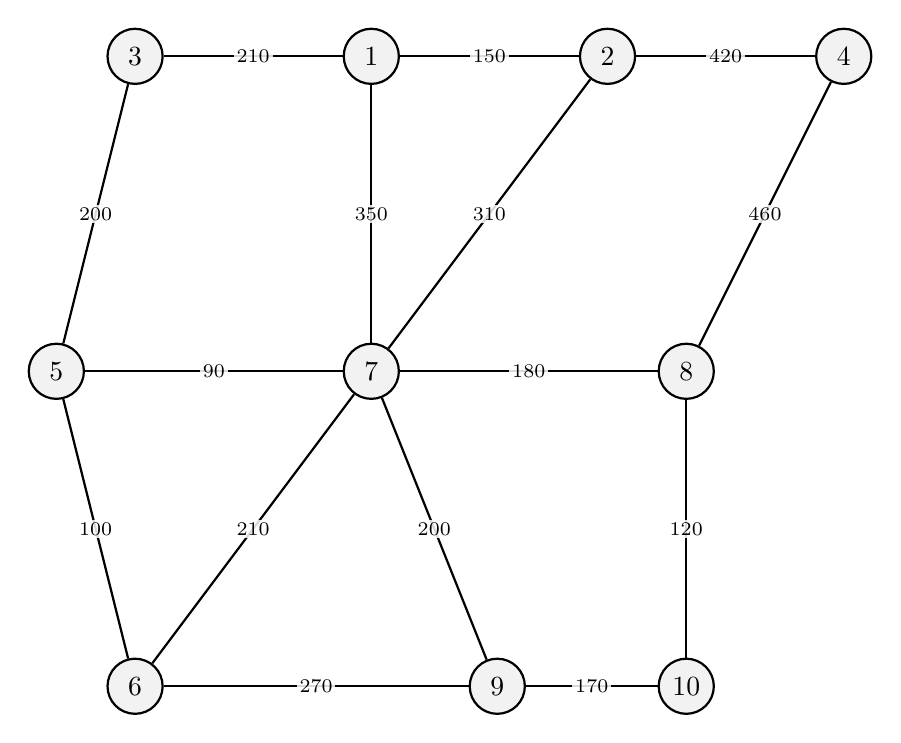
\begin{tikzpicture}[baseline, >={Stealth[length=2mm]},
  netnode/.style={circle, draw, thick, fill=gray!10, minimum size=7mm, inner sep=1pt},
  link/.style={thick},
  linklabel/.style={font=\scriptsize, inner sep=1pt, fill=white, fill opacity=0.85, text opacity=1}]
\node[netnode] (S1) at (4.000,8.000) {1};
\node[netnode] (S2) at (7.000,8.000) {2};
\node[netnode] (S3) at (1.000,8.000) {3};
\node[netnode] (S4) at (10.000,8.000) {4};
\node[netnode] (S5) at (0.000,4.000) {5};
\node[netnode] (S6) at (1.000,0.000) {6};
\node[netnode] (S7) at (4.000,4.000) {7};
\node[netnode] (S8) at (8.000,4.000) {8};
\node[netnode] (S9) at (5.600,0.000) {9};
\node[netnode] (S10) at (8.000,0.000) {10};
\draw[link] (S1) to node[linklabel] {150} (S2);
\draw[link] (S1) to node[linklabel] {210} (S3);
\draw[link] (S1) to node[linklabel] {350} (S7);
\draw[link] (S2) to node[linklabel] {420} (S4);
\draw[link] (S2) to node[linklabel] {310} (S7);
\draw[link] (S3) to node[linklabel] {200} (S5);
\draw[link] (S4) to node[linklabel] {460} (S8);
\draw[link] (S5) to node[linklabel] {100} (S6);
\draw[link] (S5) to node[linklabel] {90} (S7);
\draw[link] (S6) to node[linklabel] {210} (S7);
\draw[link] (S6) to node[linklabel] {270} (S9);
\draw[link] (S7) to node[linklabel] {180} (S8);
\draw[link] (S7) to node[linklabel] {200} (S9);
\draw[link] (S8) to node[linklabel] {120} (S10);
\draw[link] (S9) to node[linklabel] {170} (S10);
\end{tikzpicture}
\end{adjustbox}\end{center}
\section*{Performance Parameters}
\begin{center}\begin{tabular}{lr}
\toprule
Highest link load & 61 Gb/s \\
Highest used FSU & 178 / 320 \\
Total used FSUs & 174 \\
Transponder cost & 87.0 \\
\midrule
SC-DP-QPSK transponders & 58 \\
SC-DP-16QAM transponders & 0 \\
DP-16QAM transponders & 0 \\
\bottomrule
\end{tabular}\end{center}
\clearpage
\section*{Link Load Map}
\begin{center}\begin{adjustbox}{max width=\linewidth}
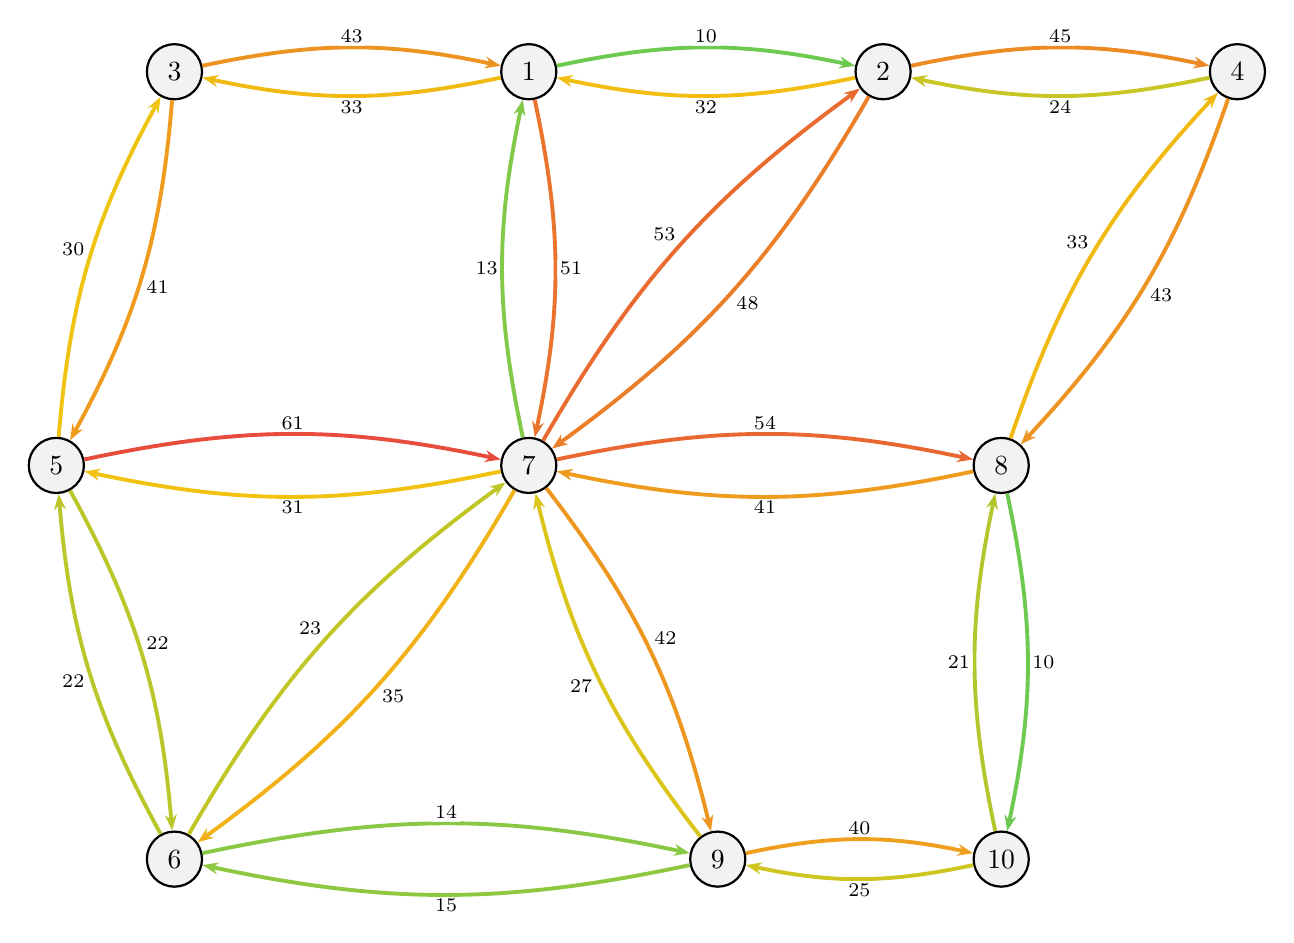
\begin{tikzpicture}[baseline, >={Stealth[length=2mm]},
  netnode/.style={circle, draw, thick, fill=gray!10, minimum size=7mm, inner sep=1pt},
  link/.style={line width=1.4pt},
  linklabel/.style={font=\scriptsize, inner sep=1pt, fill=white, fill opacity=0.85, text opacity=1}]
\node[netnode] (S1) at (6.000,10.000) {1};
\node[netnode] (S2) at (10.500,10.000) {2};
\node[netnode] (S3) at (1.500,10.000) {3};
\node[netnode] (S4) at (15.000,10.000) {4};
\node[netnode] (S5) at (0.000,5.000) {5};
\node[netnode] (S6) at (1.500,0.000) {6};
\node[netnode] (S7) at (6.000,5.000) {7};
\node[netnode] (S8) at (12.000,5.000) {8};
\node[netnode] (S9) at (8.400,0.000) {9};
\node[netnode] (S10) at (12.000,0.000) {10};
\draw[link, ->, draw={rgb,255:red,110;green,201;blue,81}] (S1) to[bend left=12] node[linklabel, auto] {10} (S2);
\draw[link, ->, draw={rgb,255:red,240;green,186;blue,19}] (S1) to[bend left=12] node[linklabel, auto] {33} (S3);
\draw[link, ->, draw={rgb,255:red,234;green,115;blue,45}] (S1) to[bend left=12] node[linklabel, auto] {51} (S7);
\draw[link, ->, draw={rgb,255:red,241;green,190;blue,17}] (S2) to[bend left=12] node[linklabel, auto] {32} (S1);
\draw[link, ->, draw={rgb,255:red,236;green,139;blue,36}] (S2) to[bend left=12] node[linklabel, auto] {45} (S4);
\draw[link, ->, draw={rgb,255:red,235;green,127;blue,41}] (S2) to[bend left=12] node[linklabel, auto] {48} (S7);
\draw[link, ->, draw={rgb,255:red,237;green,147;blue,33}] (S3) to[bend left=12] node[linklabel, auto] {43} (S1);
\draw[link, ->, draw={rgb,255:red,238;green,155;blue,30}] (S3) to[bend left=12] node[linklabel, auto] {41} (S5);
\draw[link, ->, draw={rgb,255:red,199;green,198;blue,36}] (S4) to[bend left=12] node[linklabel, auto] {24} (S2);
\draw[link, ->, draw={rgb,255:red,237;green,147;blue,33}] (S4) to[bend left=12] node[linklabel, auto] {43} (S8);
\draw[link, ->, draw={rgb,255:red,238;green,196;blue,17}] (S5) to[bend left=12] node[linklabel, auto] {30} (S3);
\draw[link, ->, draw={rgb,255:red,187;green,198;blue,42}] (S5) to[bend left=12] node[linklabel, auto] {22} (S6);
\draw[link, ->, draw={rgb,255:red,231;green,76;blue,60}] (S5) to[bend left=12] node[linklabel, auto] {61} (S7);
\draw[link, ->, draw={rgb,255:red,187;green,198;blue,42}] (S6) to[bend left=12] node[linklabel, auto] {22} (S5);
\draw[link, ->, draw={rgb,255:red,193;green,198;blue,39}] (S6) to[bend left=12] node[linklabel, auto] {23} (S7);
\draw[link, ->, draw={rgb,255:red,136;green,200;blue,68}] (S6) to[bend left=12] node[linklabel, auto] {14} (S9);
\draw[link, ->, draw={rgb,255:red,129;green,201;blue,71}] (S7) to[bend left=12] node[linklabel, auto] {13} (S1);
\draw[link, ->, draw={rgb,255:red,234;green,107;blue,48}] (S7) to[bend left=12] node[linklabel, auto] {53} (S2);
\draw[link, ->, draw={rgb,255:red,241;green,194;blue,16}] (S7) to[bend left=12] node[linklabel, auto] {31} (S5);
\draw[link, ->, draw={rgb,255:red,240;green,178;blue,22}] (S7) to[bend left=12] node[linklabel, auto] {35} (S6);
\draw[link, ->, draw={rgb,255:red,233;green,104;blue,50}] (S7) to[bend left=12] node[linklabel, auto] {54} (S8);
\draw[link, ->, draw={rgb,255:red,237;green,151;blue,32}] (S7) to[bend left=12] node[linklabel, auto] {42} (S9);
\draw[link, ->, draw={rgb,255:red,240;green,186;blue,19}] (S8) to[bend left=12] node[linklabel, auto] {33} (S4);
\draw[link, ->, draw={rgb,255:red,238;green,155;blue,30}] (S8) to[bend left=12] node[linklabel, auto] {41} (S7);
\draw[link, ->, draw={rgb,255:red,110;green,201;blue,81}] (S8) to[bend left=12] node[linklabel, auto] {10} (S10);
\draw[link, ->, draw={rgb,255:red,142;green,200;blue,65}] (S9) to[bend left=12] node[linklabel, auto] {15} (S6);
\draw[link, ->, draw={rgb,255:red,219;green,197;blue,26}] (S9) to[bend left=12] node[linklabel, auto] {27} (S7);
\draw[link, ->, draw={rgb,255:red,238;green,159;blue,29}] (S9) to[bend left=12] node[linklabel, auto] {40} (S10);
\draw[link, ->, draw={rgb,255:red,180;green,198;blue,46}] (S10) to[bend left=12] node[linklabel, auto] {21} (S8);
\draw[link, ->, draw={rgb,255:red,206;green,197;blue,33}] (S10) to[bend left=12] node[linklabel, auto] {25} (S9);
\end{tikzpicture}
\end{adjustbox}\end{center}
\begin{center}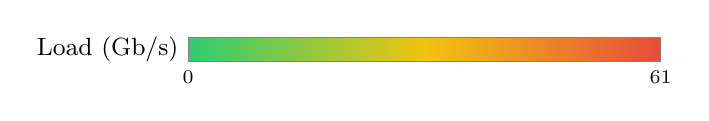
\begin{tikzpicture}
\definecolor{scalelow}{RGB}{46,204,113}\definecolor{scalemid}{RGB}{241,196,15}\definecolor{scalehigh}{RGB}{231,76,60}
\shade[left color=scalelow, right color=scalemid] (0,0) rectangle (3,0.3);
\shade[left color=scalemid, right color=scalehigh] (3,0) rectangle (6,0.3);
\draw[gray] (0,0) rectangle (6,0.3);
\node[below, font=\scriptsize] at (0,0) {0};
\node[below, font=\scriptsize] at (6,0) {61};
\node[left, font=\small] at (0,0.15) {Load (Gb/s)};
\end{tikzpicture}\end{center}
\section*{Link Load Distribution}

\begin{center}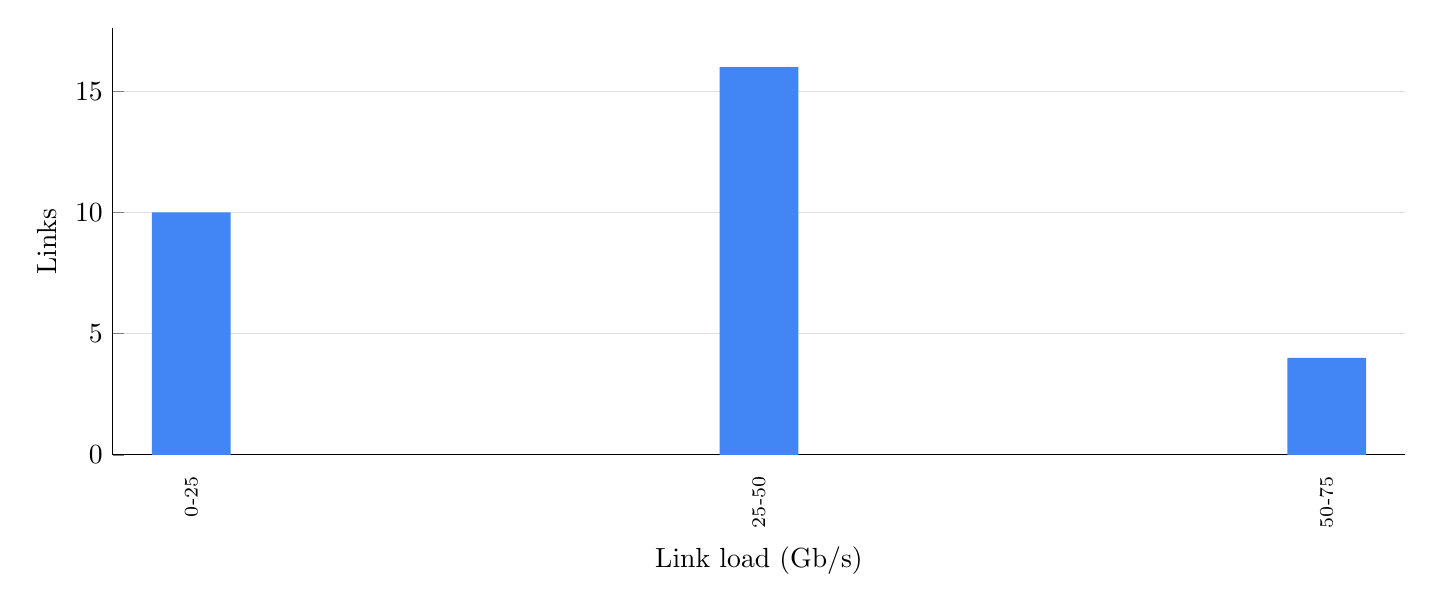
\begin{tikzpicture}
\begin{axis}[
  ybar, bar width=1.000cm, width=18.000cm, height=7cm,
  ymin=0, ymajorgrids, grid style={gray!25}, axis lines*=left,
  enlarge x limits={abs=1.000cm}, xtick=data, major x tick style={draw=none},
  x tick label style={rotate=90, font=\scriptsize, /pgf/number format/1000 sep=},
  legend style={at={(0.5,-0.3)}, anchor=north, legend columns=-1, draw=none},
  ylabel={Links},
  xlabel={Link load (Gb/s)},
  symbolic x coords={0-25,25-50,50-75}]
\addplot[fill={rgb,255:red,66;green,133;blue,244}, draw=none] coordinates {(0-25,10.000) (25-50,16.000) (50-75,4.000) };
\end{axis}
\end{tikzpicture}\end{center}
\clearpage
\section*{Spectrum Occupancy}
\begin{center}\begin{adjustbox}{max width=\linewidth}
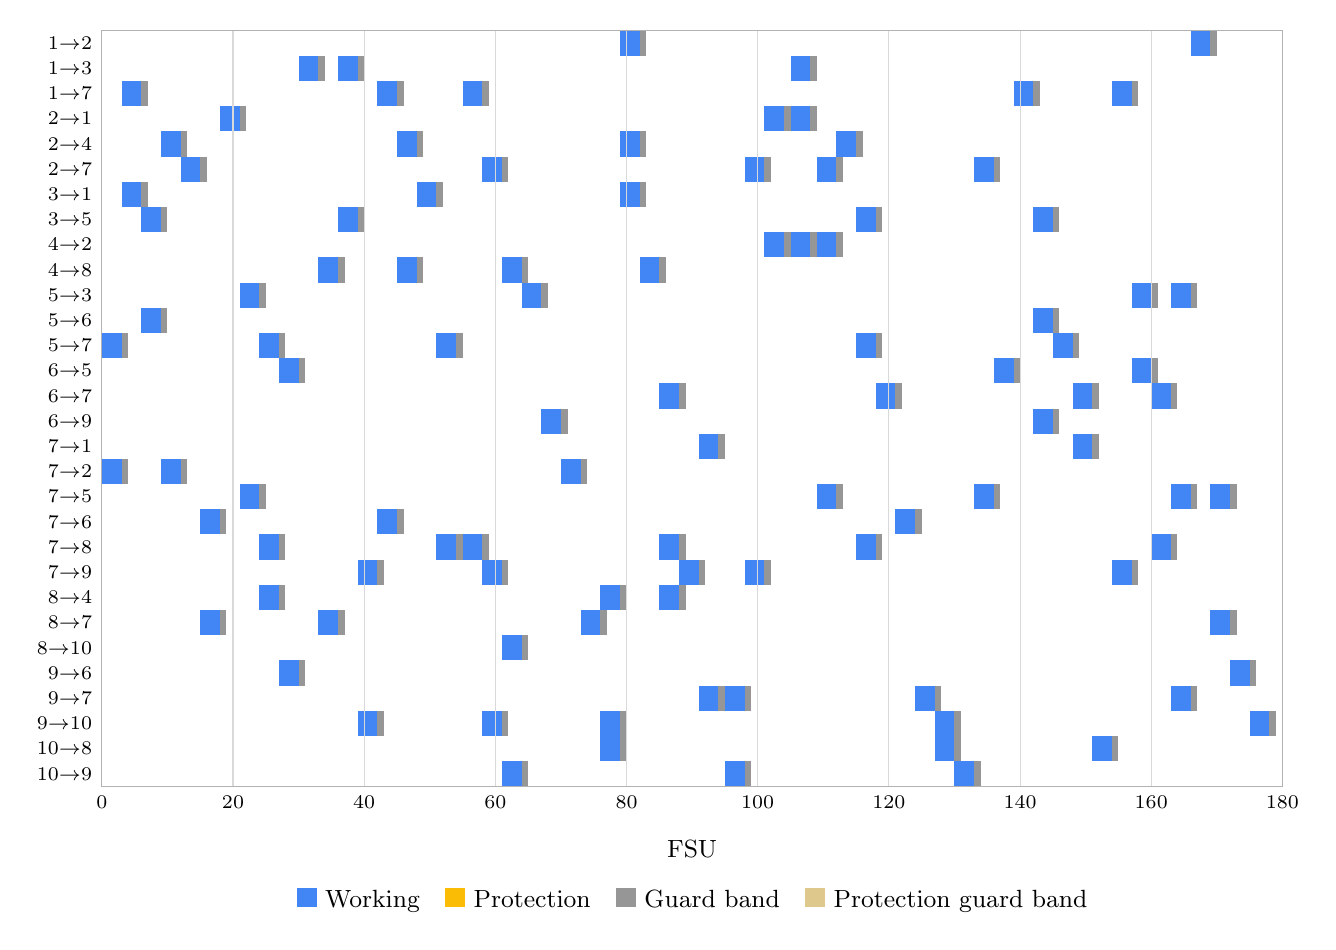
\begin{tikzpicture}[x=0.0833cm, y=-0.32cm]
\fill[fill={rgb,255:red,66;green,133;blue,244}] (79,0) rectangle (82,1);
\fill[fill={rgb,255:red,150;green,150;blue,150}] (82,0) rectangle (83,1);
\fill[fill={rgb,255:red,66;green,133;blue,244}] (166,0) rectangle (169,1);
\fill[fill={rgb,255:red,150;green,150;blue,150}] (169,0) rectangle (170,1);
\node[left, font=\scriptsize] at (0,0.5) {1\(\to\)2};
\fill[fill={rgb,255:red,66;green,133;blue,244}] (30,1) rectangle (33,2);
\fill[fill={rgb,255:red,150;green,150;blue,150}] (33,1) rectangle (34,2);
\fill[fill={rgb,255:red,66;green,133;blue,244}] (36,1) rectangle (39,2);
\fill[fill={rgb,255:red,150;green,150;blue,150}] (39,1) rectangle (40,2);
\fill[fill={rgb,255:red,66;green,133;blue,244}] (105,1) rectangle (108,2);
\fill[fill={rgb,255:red,150;green,150;blue,150}] (108,1) rectangle (109,2);
\node[left, font=\scriptsize] at (0,1.5) {1\(\to\)3};
\fill[fill={rgb,255:red,66;green,133;blue,244}] (3,2) rectangle (6,3);
\fill[fill={rgb,255:red,150;green,150;blue,150}] (6,2) rectangle (7,3);
\fill[fill={rgb,255:red,66;green,133;blue,244}] (42,2) rectangle (45,3);
\fill[fill={rgb,255:red,150;green,150;blue,150}] (45,2) rectangle (46,3);
\fill[fill={rgb,255:red,66;green,133;blue,244}] (55,2) rectangle (58,3);
\fill[fill={rgb,255:red,150;green,150;blue,150}] (58,2) rectangle (59,3);
\fill[fill={rgb,255:red,66;green,133;blue,244}] (139,2) rectangle (142,3);
\fill[fill={rgb,255:red,150;green,150;blue,150}] (142,2) rectangle (143,3);
\fill[fill={rgb,255:red,66;green,133;blue,244}] (154,2) rectangle (157,3);
\fill[fill={rgb,255:red,150;green,150;blue,150}] (157,2) rectangle (158,3);
\node[left, font=\scriptsize] at (0,2.5) {1\(\to\)7};
\fill[fill={rgb,255:red,66;green,133;blue,244}] (18,3) rectangle (21,4);
\fill[fill={rgb,255:red,150;green,150;blue,150}] (21,3) rectangle (22,4);
\fill[fill={rgb,255:red,66;green,133;blue,244}] (101,3) rectangle (104,4);
\fill[fill={rgb,255:red,150;green,150;blue,150}] (104,3) rectangle (105,4);
\fill[fill={rgb,255:red,66;green,133;blue,244}] (105,3) rectangle (108,4);
\fill[fill={rgb,255:red,150;green,150;blue,150}] (108,3) rectangle (109,4);
\node[left, font=\scriptsize] at (0,3.5) {2\(\to\)1};
\fill[fill={rgb,255:red,66;green,133;blue,244}] (9,4) rectangle (12,5);
\fill[fill={rgb,255:red,150;green,150;blue,150}] (12,4) rectangle (13,5);
\fill[fill={rgb,255:red,66;green,133;blue,244}] (45,4) rectangle (48,5);
\fill[fill={rgb,255:red,150;green,150;blue,150}] (48,4) rectangle (49,5);
\fill[fill={rgb,255:red,66;green,133;blue,244}] (79,4) rectangle (82,5);
\fill[fill={rgb,255:red,150;green,150;blue,150}] (82,4) rectangle (83,5);
\fill[fill={rgb,255:red,66;green,133;blue,244}] (112,4) rectangle (115,5);
\fill[fill={rgb,255:red,150;green,150;blue,150}] (115,4) rectangle (116,5);
\node[left, font=\scriptsize] at (0,4.5) {2\(\to\)4};
\fill[fill={rgb,255:red,66;green,133;blue,244}] (12,5) rectangle (15,6);
\fill[fill={rgb,255:red,150;green,150;blue,150}] (15,5) rectangle (16,6);
\fill[fill={rgb,255:red,66;green,133;blue,244}] (58,5) rectangle (61,6);
\fill[fill={rgb,255:red,150;green,150;blue,150}] (61,5) rectangle (62,6);
\fill[fill={rgb,255:red,66;green,133;blue,244}] (98,5) rectangle (101,6);
\fill[fill={rgb,255:red,150;green,150;blue,150}] (101,5) rectangle (102,6);
\fill[fill={rgb,255:red,66;green,133;blue,244}] (109,5) rectangle (112,6);
\fill[fill={rgb,255:red,150;green,150;blue,150}] (112,5) rectangle (113,6);
\fill[fill={rgb,255:red,66;green,133;blue,244}] (133,5) rectangle (136,6);
\fill[fill={rgb,255:red,150;green,150;blue,150}] (136,5) rectangle (137,6);
\node[left, font=\scriptsize] at (0,5.5) {2\(\to\)7};
\fill[fill={rgb,255:red,66;green,133;blue,244}] (3,6) rectangle (6,7);
\fill[fill={rgb,255:red,150;green,150;blue,150}] (6,6) rectangle (7,7);
\fill[fill={rgb,255:red,66;green,133;blue,244}] (48,6) rectangle (51,7);
\fill[fill={rgb,255:red,150;green,150;blue,150}] (51,6) rectangle (52,7);
\fill[fill={rgb,255:red,66;green,133;blue,244}] (79,6) rectangle (82,7);
\fill[fill={rgb,255:red,150;green,150;blue,150}] (82,6) rectangle (83,7);
\node[left, font=\scriptsize] at (0,6.5) {3\(\to\)1};
\fill[fill={rgb,255:red,66;green,133;blue,244}] (6,7) rectangle (9,8);
\fill[fill={rgb,255:red,150;green,150;blue,150}] (9,7) rectangle (10,8);
\fill[fill={rgb,255:red,66;green,133;blue,244}] (36,7) rectangle (39,8);
\fill[fill={rgb,255:red,150;green,150;blue,150}] (39,7) rectangle (40,8);
\fill[fill={rgb,255:red,66;green,133;blue,244}] (115,7) rectangle (118,8);
\fill[fill={rgb,255:red,150;green,150;blue,150}] (118,7) rectangle (119,8);
\fill[fill={rgb,255:red,66;green,133;blue,244}] (142,7) rectangle (145,8);
\fill[fill={rgb,255:red,150;green,150;blue,150}] (145,7) rectangle (146,8);
\node[left, font=\scriptsize] at (0,7.5) {3\(\to\)5};
\fill[fill={rgb,255:red,66;green,133;blue,244}] (101,8) rectangle (104,9);
\fill[fill={rgb,255:red,150;green,150;blue,150}] (104,8) rectangle (105,9);
\fill[fill={rgb,255:red,66;green,133;blue,244}] (105,8) rectangle (108,9);
\fill[fill={rgb,255:red,150;green,150;blue,150}] (108,8) rectangle (109,9);
\fill[fill={rgb,255:red,66;green,133;blue,244}] (109,8) rectangle (112,9);
\fill[fill={rgb,255:red,150;green,150;blue,150}] (112,8) rectangle (113,9);
\node[left, font=\scriptsize] at (0,8.5) {4\(\to\)2};
\fill[fill={rgb,255:red,66;green,133;blue,244}] (33,9) rectangle (36,10);
\fill[fill={rgb,255:red,150;green,150;blue,150}] (36,9) rectangle (37,10);
\fill[fill={rgb,255:red,66;green,133;blue,244}] (45,9) rectangle (48,10);
\fill[fill={rgb,255:red,150;green,150;blue,150}] (48,9) rectangle (49,10);
\fill[fill={rgb,255:red,66;green,133;blue,244}] (61,9) rectangle (64,10);
\fill[fill={rgb,255:red,150;green,150;blue,150}] (64,9) rectangle (65,10);
\fill[fill={rgb,255:red,66;green,133;blue,244}] (82,9) rectangle (85,10);
\fill[fill={rgb,255:red,150;green,150;blue,150}] (85,9) rectangle (86,10);
\node[left, font=\scriptsize] at (0,9.5) {4\(\to\)8};
\fill[fill={rgb,255:red,66;green,133;blue,244}] (21,10) rectangle (24,11);
\fill[fill={rgb,255:red,150;green,150;blue,150}] (24,10) rectangle (25,11);
\fill[fill={rgb,255:red,66;green,133;blue,244}] (64,10) rectangle (67,11);
\fill[fill={rgb,255:red,150;green,150;blue,150}] (67,10) rectangle (68,11);
\fill[fill={rgb,255:red,66;green,133;blue,244}] (157,10) rectangle (160,11);
\fill[fill={rgb,255:red,150;green,150;blue,150}] (160,10) rectangle (161,11);
\fill[fill={rgb,255:red,66;green,133;blue,244}] (163,10) rectangle (166,11);
\fill[fill={rgb,255:red,150;green,150;blue,150}] (166,10) rectangle (167,11);
\node[left, font=\scriptsize] at (0,10.5) {5\(\to\)3};
\fill[fill={rgb,255:red,66;green,133;blue,244}] (6,11) rectangle (9,12);
\fill[fill={rgb,255:red,150;green,150;blue,150}] (9,11) rectangle (10,12);
\fill[fill={rgb,255:red,66;green,133;blue,244}] (142,11) rectangle (145,12);
\fill[fill={rgb,255:red,150;green,150;blue,150}] (145,11) rectangle (146,12);
\node[left, font=\scriptsize] at (0,11.5) {5\(\to\)6};
\fill[fill={rgb,255:red,66;green,133;blue,244}] (0,12) rectangle (3,13);
\fill[fill={rgb,255:red,150;green,150;blue,150}] (3,12) rectangle (4,13);
\fill[fill={rgb,255:red,66;green,133;blue,244}] (24,12) rectangle (27,13);
\fill[fill={rgb,255:red,150;green,150;blue,150}] (27,12) rectangle (28,13);
\fill[fill={rgb,255:red,66;green,133;blue,244}] (51,12) rectangle (54,13);
\fill[fill={rgb,255:red,150;green,150;blue,150}] (54,12) rectangle (55,13);
\fill[fill={rgb,255:red,66;green,133;blue,244}] (115,12) rectangle (118,13);
\fill[fill={rgb,255:red,150;green,150;blue,150}] (118,12) rectangle (119,13);
\fill[fill={rgb,255:red,66;green,133;blue,244}] (145,12) rectangle (148,13);
\fill[fill={rgb,255:red,150;green,150;blue,150}] (148,12) rectangle (149,13);
\node[left, font=\scriptsize] at (0,12.5) {5\(\to\)7};
\fill[fill={rgb,255:red,66;green,133;blue,244}] (27,13) rectangle (30,14);
\fill[fill={rgb,255:red,150;green,150;blue,150}] (30,13) rectangle (31,14);
\fill[fill={rgb,255:red,66;green,133;blue,244}] (136,13) rectangle (139,14);
\fill[fill={rgb,255:red,150;green,150;blue,150}] (139,13) rectangle (140,14);
\fill[fill={rgb,255:red,66;green,133;blue,244}] (157,13) rectangle (160,14);
\fill[fill={rgb,255:red,150;green,150;blue,150}] (160,13) rectangle (161,14);
\node[left, font=\scriptsize] at (0,13.5) {6\(\to\)5};
\fill[fill={rgb,255:red,66;green,133;blue,244}] (85,14) rectangle (88,15);
\fill[fill={rgb,255:red,150;green,150;blue,150}] (88,14) rectangle (89,15);
\fill[fill={rgb,255:red,66;green,133;blue,244}] (118,14) rectangle (121,15);
\fill[fill={rgb,255:red,150;green,150;blue,150}] (121,14) rectangle (122,15);
\fill[fill={rgb,255:red,66;green,133;blue,244}] (148,14) rectangle (151,15);
\fill[fill={rgb,255:red,150;green,150;blue,150}] (151,14) rectangle (152,15);
\fill[fill={rgb,255:red,66;green,133;blue,244}] (160,14) rectangle (163,15);
\fill[fill={rgb,255:red,150;green,150;blue,150}] (163,14) rectangle (164,15);
\node[left, font=\scriptsize] at (0,14.5) {6\(\to\)7};
\fill[fill={rgb,255:red,66;green,133;blue,244}] (67,15) rectangle (70,16);
\fill[fill={rgb,255:red,150;green,150;blue,150}] (70,15) rectangle (71,16);
\fill[fill={rgb,255:red,66;green,133;blue,244}] (142,15) rectangle (145,16);
\fill[fill={rgb,255:red,150;green,150;blue,150}] (145,15) rectangle (146,16);
\node[left, font=\scriptsize] at (0,15.5) {6\(\to\)9};
\fill[fill={rgb,255:red,66;green,133;blue,244}] (91,16) rectangle (94,17);
\fill[fill={rgb,255:red,150;green,150;blue,150}] (94,16) rectangle (95,17);
\fill[fill={rgb,255:red,66;green,133;blue,244}] (148,16) rectangle (151,17);
\fill[fill={rgb,255:red,150;green,150;blue,150}] (151,16) rectangle (152,17);
\node[left, font=\scriptsize] at (0,16.5) {7\(\to\)1};
\fill[fill={rgb,255:red,66;green,133;blue,244}] (0,17) rectangle (3,18);
\fill[fill={rgb,255:red,150;green,150;blue,150}] (3,17) rectangle (4,18);
\fill[fill={rgb,255:red,66;green,133;blue,244}] (9,17) rectangle (12,18);
\fill[fill={rgb,255:red,150;green,150;blue,150}] (12,17) rectangle (13,18);
\fill[fill={rgb,255:red,66;green,133;blue,244}] (70,17) rectangle (73,18);
\fill[fill={rgb,255:red,150;green,150;blue,150}] (73,17) rectangle (74,18);
\node[left, font=\scriptsize] at (0,17.5) {7\(\to\)2};
\fill[fill={rgb,255:red,66;green,133;blue,244}] (21,18) rectangle (24,19);
\fill[fill={rgb,255:red,150;green,150;blue,150}] (24,18) rectangle (25,19);
\fill[fill={rgb,255:red,66;green,133;blue,244}] (109,18) rectangle (112,19);
\fill[fill={rgb,255:red,150;green,150;blue,150}] (112,18) rectangle (113,19);
\fill[fill={rgb,255:red,66;green,133;blue,244}] (133,18) rectangle (136,19);
\fill[fill={rgb,255:red,150;green,150;blue,150}] (136,18) rectangle (137,19);
\fill[fill={rgb,255:red,66;green,133;blue,244}] (163,18) rectangle (166,19);
\fill[fill={rgb,255:red,150;green,150;blue,150}] (166,18) rectangle (167,19);
\fill[fill={rgb,255:red,66;green,133;blue,244}] (169,18) rectangle (172,19);
\fill[fill={rgb,255:red,150;green,150;blue,150}] (172,18) rectangle (173,19);
\node[left, font=\scriptsize] at (0,18.5) {7\(\to\)5};
\fill[fill={rgb,255:red,66;green,133;blue,244}] (15,19) rectangle (18,20);
\fill[fill={rgb,255:red,150;green,150;blue,150}] (18,19) rectangle (19,20);
\fill[fill={rgb,255:red,66;green,133;blue,244}] (42,19) rectangle (45,20);
\fill[fill={rgb,255:red,150;green,150;blue,150}] (45,19) rectangle (46,20);
\fill[fill={rgb,255:red,66;green,133;blue,244}] (121,19) rectangle (124,20);
\fill[fill={rgb,255:red,150;green,150;blue,150}] (124,19) rectangle (125,20);
\node[left, font=\scriptsize] at (0,19.5) {7\(\to\)6};
\fill[fill={rgb,255:red,66;green,133;blue,244}] (24,20) rectangle (27,21);
\fill[fill={rgb,255:red,150;green,150;blue,150}] (27,20) rectangle (28,21);
\fill[fill={rgb,255:red,66;green,133;blue,244}] (51,20) rectangle (54,21);
\fill[fill={rgb,255:red,150;green,150;blue,150}] (54,20) rectangle (55,21);
\fill[fill={rgb,255:red,66;green,133;blue,244}] (55,20) rectangle (58,21);
\fill[fill={rgb,255:red,150;green,150;blue,150}] (58,20) rectangle (59,21);
\fill[fill={rgb,255:red,66;green,133;blue,244}] (85,20) rectangle (88,21);
\fill[fill={rgb,255:red,150;green,150;blue,150}] (88,20) rectangle (89,21);
\fill[fill={rgb,255:red,66;green,133;blue,244}] (115,20) rectangle (118,21);
\fill[fill={rgb,255:red,150;green,150;blue,150}] (118,20) rectangle (119,21);
\fill[fill={rgb,255:red,66;green,133;blue,244}] (160,20) rectangle (163,21);
\fill[fill={rgb,255:red,150;green,150;blue,150}] (163,20) rectangle (164,21);
\node[left, font=\scriptsize] at (0,20.5) {7\(\to\)8};
\fill[fill={rgb,255:red,66;green,133;blue,244}] (39,21) rectangle (42,22);
\fill[fill={rgb,255:red,150;green,150;blue,150}] (42,21) rectangle (43,22);
\fill[fill={rgb,255:red,66;green,133;blue,244}] (58,21) rectangle (61,22);
\fill[fill={rgb,255:red,150;green,150;blue,150}] (61,21) rectangle (62,22);
\fill[fill={rgb,255:red,66;green,133;blue,244}] (88,21) rectangle (91,22);
\fill[fill={rgb,255:red,150;green,150;blue,150}] (91,21) rectangle (92,22);
\fill[fill={rgb,255:red,66;green,133;blue,244}] (98,21) rectangle (101,22);
\fill[fill={rgb,255:red,150;green,150;blue,150}] (101,21) rectangle (102,22);
\fill[fill={rgb,255:red,66;green,133;blue,244}] (154,21) rectangle (157,22);
\fill[fill={rgb,255:red,150;green,150;blue,150}] (157,21) rectangle (158,22);
\node[left, font=\scriptsize] at (0,21.5) {7\(\to\)9};
\fill[fill={rgb,255:red,66;green,133;blue,244}] (24,22) rectangle (27,23);
\fill[fill={rgb,255:red,150;green,150;blue,150}] (27,22) rectangle (28,23);
\fill[fill={rgb,255:red,66;green,133;blue,244}] (76,22) rectangle (79,23);
\fill[fill={rgb,255:red,150;green,150;blue,150}] (79,22) rectangle (80,23);
\fill[fill={rgb,255:red,66;green,133;blue,244}] (85,22) rectangle (88,23);
\fill[fill={rgb,255:red,150;green,150;blue,150}] (88,22) rectangle (89,23);
\node[left, font=\scriptsize] at (0,22.5) {8\(\to\)4};
\fill[fill={rgb,255:red,66;green,133;blue,244}] (15,23) rectangle (18,24);
\fill[fill={rgb,255:red,150;green,150;blue,150}] (18,23) rectangle (19,24);
\fill[fill={rgb,255:red,66;green,133;blue,244}] (33,23) rectangle (36,24);
\fill[fill={rgb,255:red,150;green,150;blue,150}] (36,23) rectangle (37,24);
\fill[fill={rgb,255:red,66;green,133;blue,244}] (73,23) rectangle (76,24);
\fill[fill={rgb,255:red,150;green,150;blue,150}] (76,23) rectangle (77,24);
\fill[fill={rgb,255:red,66;green,133;blue,244}] (169,23) rectangle (172,24);
\fill[fill={rgb,255:red,150;green,150;blue,150}] (172,23) rectangle (173,24);
\node[left, font=\scriptsize] at (0,23.5) {8\(\to\)7};
\fill[fill={rgb,255:red,66;green,133;blue,244}] (61,24) rectangle (64,25);
\fill[fill={rgb,255:red,150;green,150;blue,150}] (64,24) rectangle (65,25);
\node[left, font=\scriptsize] at (0,24.5) {8\(\to\)10};
\fill[fill={rgb,255:red,66;green,133;blue,244}] (27,25) rectangle (30,26);
\fill[fill={rgb,255:red,150;green,150;blue,150}] (30,25) rectangle (31,26);
\fill[fill={rgb,255:red,66;green,133;blue,244}] (172,25) rectangle (175,26);
\fill[fill={rgb,255:red,150;green,150;blue,150}] (175,25) rectangle (176,26);
\node[left, font=\scriptsize] at (0,25.5) {9\(\to\)6};
\fill[fill={rgb,255:red,66;green,133;blue,244}] (91,26) rectangle (94,27);
\fill[fill={rgb,255:red,150;green,150;blue,150}] (94,26) rectangle (95,27);
\fill[fill={rgb,255:red,66;green,133;blue,244}] (95,26) rectangle (98,27);
\fill[fill={rgb,255:red,150;green,150;blue,150}] (98,26) rectangle (99,27);
\fill[fill={rgb,255:red,66;green,133;blue,244}] (124,26) rectangle (127,27);
\fill[fill={rgb,255:red,150;green,150;blue,150}] (127,26) rectangle (128,27);
\fill[fill={rgb,255:red,66;green,133;blue,244}] (163,26) rectangle (166,27);
\fill[fill={rgb,255:red,150;green,150;blue,150}] (166,26) rectangle (167,27);
\node[left, font=\scriptsize] at (0,26.5) {9\(\to\)7};
\fill[fill={rgb,255:red,66;green,133;blue,244}] (39,27) rectangle (42,28);
\fill[fill={rgb,255:red,150;green,150;blue,150}] (42,27) rectangle (43,28);
\fill[fill={rgb,255:red,66;green,133;blue,244}] (58,27) rectangle (61,28);
\fill[fill={rgb,255:red,150;green,150;blue,150}] (61,27) rectangle (62,28);
\fill[fill={rgb,255:red,66;green,133;blue,244}] (76,27) rectangle (79,28);
\fill[fill={rgb,255:red,150;green,150;blue,150}] (79,27) rectangle (80,28);
\fill[fill={rgb,255:red,66;green,133;blue,244}] (127,27) rectangle (130,28);
\fill[fill={rgb,255:red,150;green,150;blue,150}] (130,27) rectangle (131,28);
\fill[fill={rgb,255:red,66;green,133;blue,244}] (175,27) rectangle (178,28);
\fill[fill={rgb,255:red,150;green,150;blue,150}] (178,27) rectangle (179,28);
\node[left, font=\scriptsize] at (0,27.5) {9\(\to\)10};
\fill[fill={rgb,255:red,66;green,133;blue,244}] (76,28) rectangle (79,29);
\fill[fill={rgb,255:red,150;green,150;blue,150}] (79,28) rectangle (80,29);
\fill[fill={rgb,255:red,66;green,133;blue,244}] (127,28) rectangle (130,29);
\fill[fill={rgb,255:red,150;green,150;blue,150}] (130,28) rectangle (131,29);
\fill[fill={rgb,255:red,66;green,133;blue,244}] (151,28) rectangle (154,29);
\fill[fill={rgb,255:red,150;green,150;blue,150}] (154,28) rectangle (155,29);
\node[left, font=\scriptsize] at (0,28.5) {10\(\to\)8};
\fill[fill={rgb,255:red,66;green,133;blue,244}] (61,29) rectangle (64,30);
\fill[fill={rgb,255:red,150;green,150;blue,150}] (64,29) rectangle (65,30);
\fill[fill={rgb,255:red,66;green,133;blue,244}] (95,29) rectangle (98,30);
\fill[fill={rgb,255:red,150;green,150;blue,150}] (98,29) rectangle (99,30);
\fill[fill={rgb,255:red,66;green,133;blue,244}] (130,29) rectangle (133,30);
\fill[fill={rgb,255:red,150;green,150;blue,150}] (133,29) rectangle (134,30);
\node[left, font=\scriptsize] at (0,29.5) {10\(\to\)9};
\foreach \s in {0,20,...,180} {\draw[gray!30] (\s,0) -- (\s,30); \node[below, font=\scriptsize] at (\s,30) {\s};}
\draw[gray!60] (0,0) rectangle (180,30);
\node[font=\small] at (90.0,32.5) {FSU};
\node[font=\small] at (90.0,34.5) {\textcolor[RGB]{66,133,244}{\rule{2.5mm}{2.5mm}} Working\quad \textcolor[RGB]{251,188,5}{\rule{2.5mm}{2.5mm}} Protection\quad \textcolor[RGB]{150,150,150}{\rule{2.5mm}{2.5mm}} Guard band\quad \textcolor[RGB]{222,200,140}{\rule{2.5mm}{2.5mm}} Protection guard band\quad };
\end{tikzpicture}
\end{adjustbox}\end{center}
\clearpage
\section*{Path Length Distribution}

\begin{center}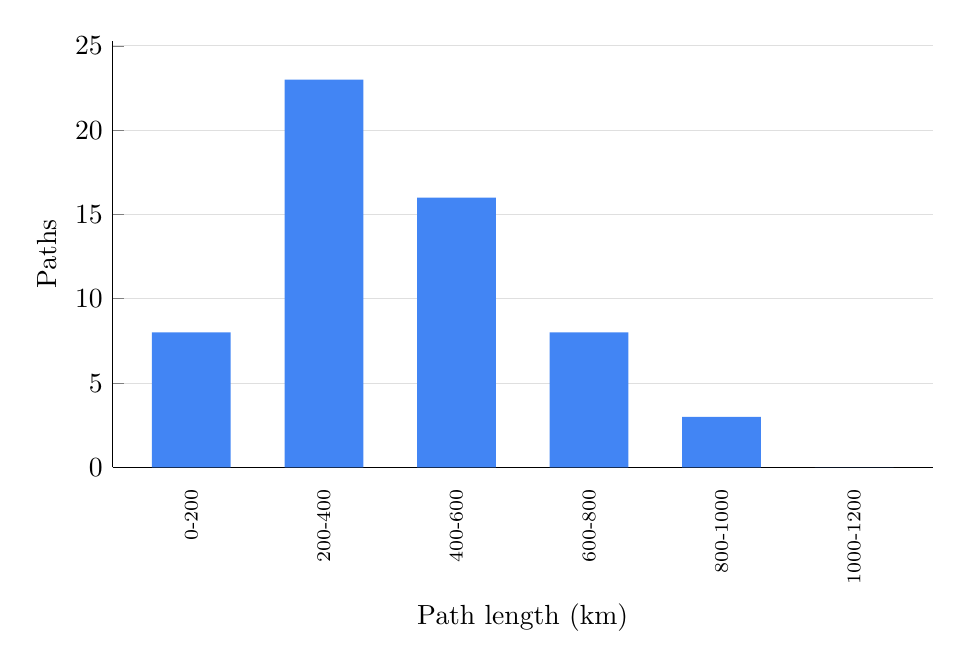
\begin{tikzpicture}
\begin{axis}[
  ybar, bar width=1.000cm, width=12.000cm, height=7cm,
  ymin=0, ymajorgrids, grid style={gray!25}, axis lines*=left,
  enlarge x limits={abs=1.000cm}, xtick=data, major x tick style={draw=none},
  x tick label style={rotate=90, font=\scriptsize, /pgf/number format/1000 sep=},
  legend style={at={(0.5,-0.3)}, anchor=north, legend columns=-1, draw=none},
  ylabel={Paths},
  xlabel={Path length (km)},
  symbolic x coords={0-200,200-400,400-600,600-800,800-1000,1000-1200,1200-1400,1400-1600,1600-1800,1800-2000}]
\addplot[fill={rgb,255:red,66;green,133;blue,244}, draw=none] coordinates {(0-200,8.000) (200-400,23.000) (400-600,16.000) (600-800,8.000) (800-1000,3.000) (1000-1200,0.000) };
\end{axis}
\end{tikzpicture}\end{center}
\clearpage
\section*{Utilization Entropy}
\begin{center}\begin{adjustbox}{max width=\linewidth}
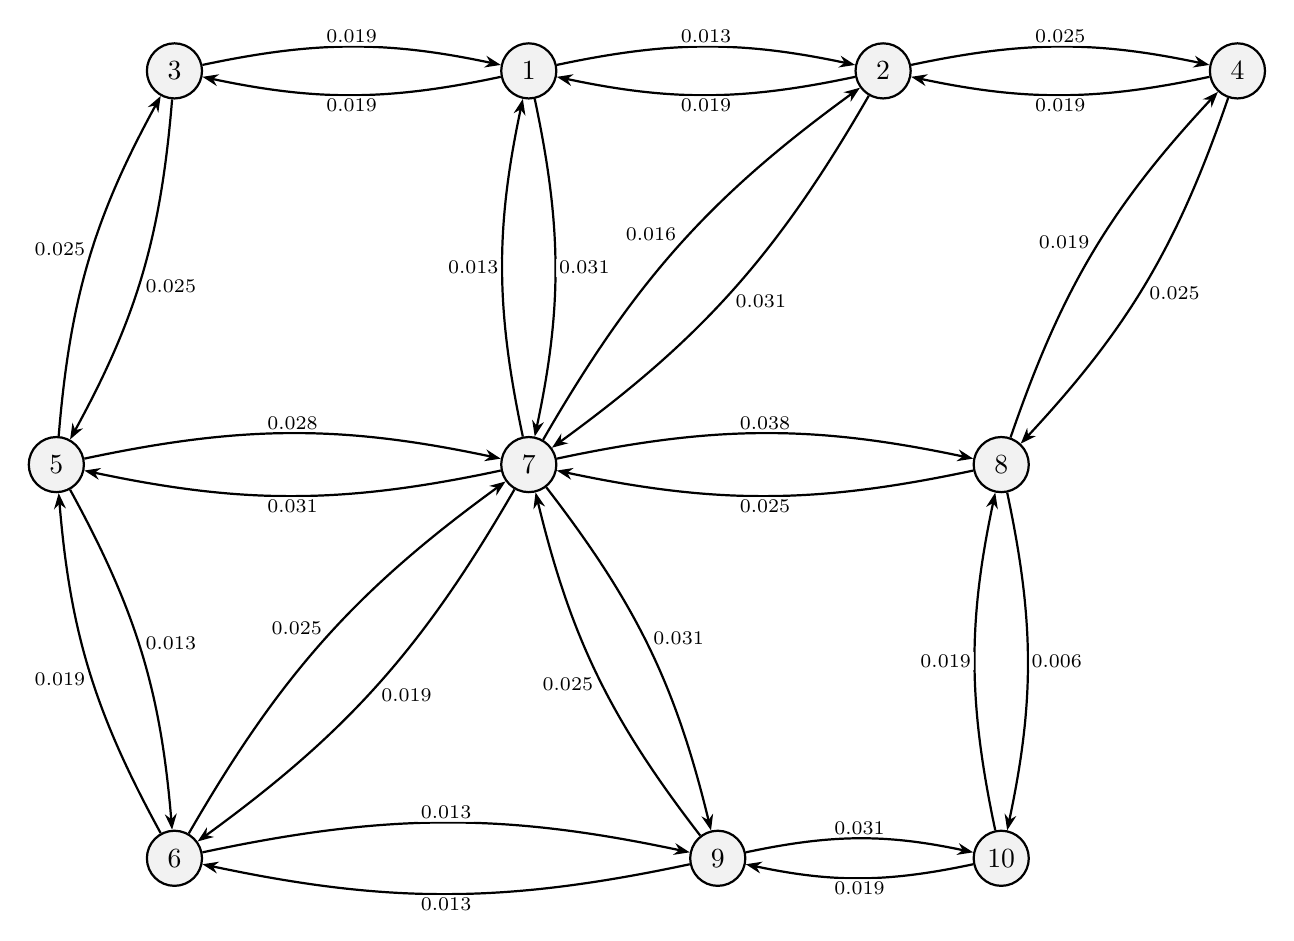
\begin{tikzpicture}[baseline, >={Stealth[length=2mm]},
  netnode/.style={circle, draw, thick, fill=gray!10, minimum size=7mm, inner sep=1pt},
  link/.style={thick},
  linklabel/.style={font=\scriptsize, inner sep=1pt, fill=white, fill opacity=0.85, text opacity=1}]
\node[netnode] (S1) at (6.000,10.000) {1};
\node[netnode] (S2) at (10.500,10.000) {2};
\node[netnode] (S3) at (1.500,10.000) {3};
\node[netnode] (S4) at (15.000,10.000) {4};
\node[netnode] (S5) at (0.000,5.000) {5};
\node[netnode] (S6) at (1.500,0.000) {6};
\node[netnode] (S7) at (6.000,5.000) {7};
\node[netnode] (S8) at (12.000,5.000) {8};
\node[netnode] (S9) at (8.400,0.000) {9};
\node[netnode] (S10) at (12.000,0.000) {10};
\draw[link, ->] (S1) to[bend left=12] node[linklabel, auto] {0.013} (S2);
\draw[link, ->] (S1) to[bend left=12] node[linklabel, auto] {0.019} (S3);
\draw[link, ->] (S1) to[bend left=12] node[linklabel, auto] {0.031} (S7);
\draw[link, ->] (S2) to[bend left=12] node[linklabel, auto] {0.019} (S1);
\draw[link, ->] (S2) to[bend left=12] node[linklabel, auto] {0.025} (S4);
\draw[link, ->] (S2) to[bend left=12] node[linklabel, auto] {0.031} (S7);
\draw[link, ->] (S3) to[bend left=12] node[linklabel, auto] {0.019} (S1);
\draw[link, ->] (S3) to[bend left=12] node[linklabel, auto] {0.025} (S5);
\draw[link, ->] (S4) to[bend left=12] node[linklabel, auto] {0.019} (S2);
\draw[link, ->] (S4) to[bend left=12] node[linklabel, auto] {0.025} (S8);
\draw[link, ->] (S5) to[bend left=12] node[linklabel, auto] {0.025} (S3);
\draw[link, ->] (S5) to[bend left=12] node[linklabel, auto] {0.013} (S6);
\draw[link, ->] (S5) to[bend left=12] node[linklabel, auto] {0.028} (S7);
\draw[link, ->] (S6) to[bend left=12] node[linklabel, auto] {0.019} (S5);
\draw[link, ->] (S6) to[bend left=12] node[linklabel, auto] {0.025} (S7);
\draw[link, ->] (S6) to[bend left=12] node[linklabel, auto] {0.013} (S9);
\draw[link, ->] (S7) to[bend left=12] node[linklabel, auto] {0.013} (S1);
\draw[link, ->] (S7) to[bend left=12] node[linklabel, auto] {0.016} (S2);
\draw[link, ->] (S7) to[bend left=12] node[linklabel, auto] {0.031} (S5);
\draw[link, ->] (S7) to[bend left=12] node[linklabel, auto] {0.019} (S6);
\draw[link, ->] (S7) to[bend left=12] node[linklabel, auto] {0.038} (S8);
\draw[link, ->] (S7) to[bend left=12] node[linklabel, auto] {0.031} (S9);
\draw[link, ->] (S8) to[bend left=12] node[linklabel, auto] {0.019} (S4);
\draw[link, ->] (S8) to[bend left=12] node[linklabel, auto] {0.025} (S7);
\draw[link, ->] (S8) to[bend left=12] node[linklabel, auto] {0.006} (S10);
\draw[link, ->] (S9) to[bend left=12] node[linklabel, auto] {0.013} (S6);
\draw[link, ->] (S9) to[bend left=12] node[linklabel, auto] {0.025} (S7);
\draw[link, ->] (S9) to[bend left=12] node[linklabel, auto] {0.031} (S10);
\draw[link, ->] (S10) to[bend left=12] node[linklabel, auto] {0.019} (S8);
\draw[link, ->] (S10) to[bend left=12] node[linklabel, auto] {0.019} (S9);
\end{tikzpicture}
\end{adjustbox}\end{center}

\begin{center}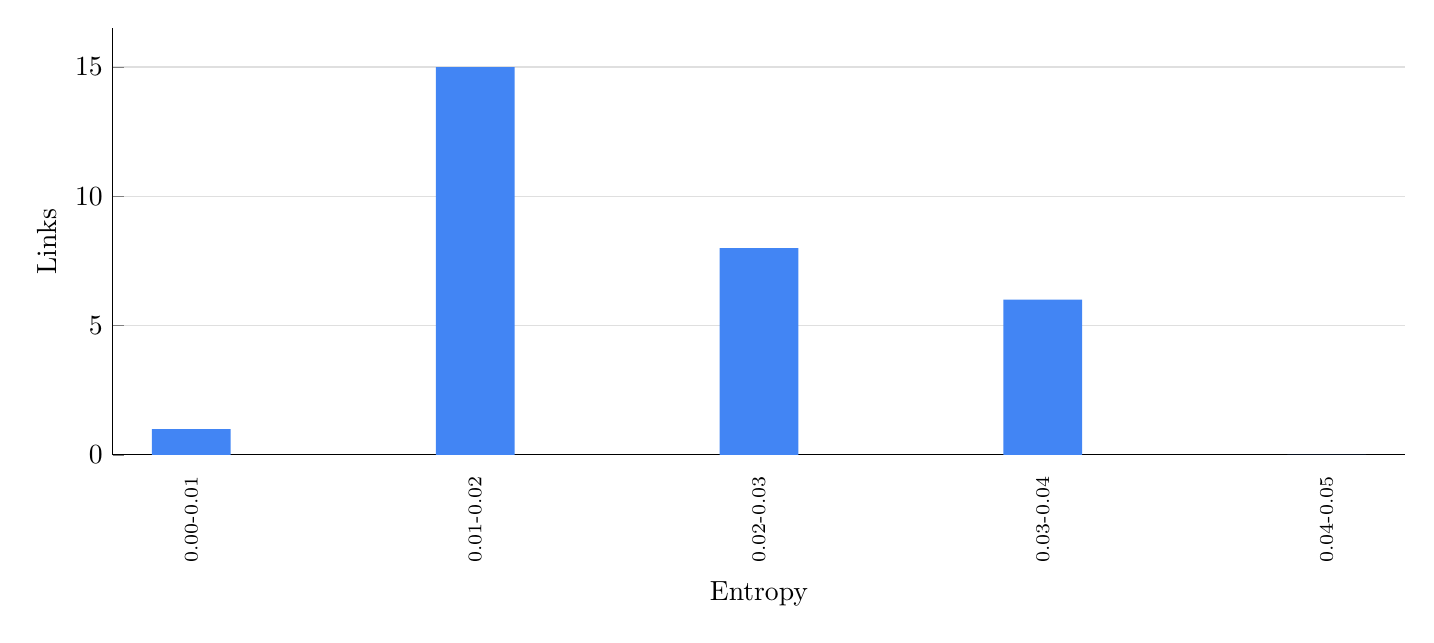
\begin{tikzpicture}
\begin{axis}[
  ybar, bar width=1.000cm, width=18.000cm, height=7cm,
  ymin=0, ymajorgrids, grid style={gray!25}, axis lines*=left,
  enlarge x limits={abs=1.000cm}, xtick=data, major x tick style={draw=none},
  x tick label style={rotate=90, font=\scriptsize, /pgf/number format/1000 sep=},
  legend style={at={(0.5,-0.3)}, anchor=north, legend columns=-1, draw=none},
  ylabel={Links},
  xlabel={Entropy},
  symbolic x coords={0.00-0.01,0.01-0.02,0.02-0.03,0.03-0.04,0.04-0.05,0.05-0.06,0.06-0.07,0.07-0.08,0.08-0.09,0.09-0.10,0.10-0.11,0.11-0.12,0.12-0.13,0.13-0.14,0.14-0.15,0.15-0.16,0.16-0.17,0.17-0.18,0.18-0.19,0.19-0.20,0.20-0.21,0.21-0.22,0.22-0.23,0.23-0.24,0.24-0.25,0.25-0.26,0.26-0.27,0.27-0.28,0.28-0.29,0.29-0.30,0.30-0.31,0.31-0.32,0.32-0.33,0.33-0.34,0.34-0.35,0.35-0.36,0.36-0.37,0.37-0.38,0.38-0.39,0.39-0.40,0.40-0.41,0.41-0.42,0.42-0.43,0.43-0.44,0.44-0.45,0.45-0.46,0.46-0.47,0.47-0.48,0.48-0.49,0.49-0.50,0.50-0.51,0.51-0.52,0.52-0.53,0.53-0.54,0.54-0.55,0.55-0.56,0.56-0.57,0.57-0.58,0.58-0.59,0.59-0.60,0.60-0.61,0.61-0.62,0.62-0.63,0.63-0.64,0.64-0.65,0.65-0.66,0.66-0.67,0.67-0.68,0.68-0.69,0.69-0.70,0.70-0.71,0.71-0.72,0.72-0.73,0.73-0.74,0.74-0.75,0.75-0.76,0.76-0.77,0.77-0.78,0.78-0.79,0.79-0.80,0.80-0.81,0.81-0.82,0.82-0.83,0.83-0.84,0.84-0.85,0.85-0.86,0.86-0.87,0.87-0.88,0.88-0.89,0.89-0.90,0.90-0.91,0.91-0.92,0.92-0.93,0.93-0.94,0.94-0.95,0.95-0.96,0.96-0.97,0.97-0.98,0.98-0.99,0.99-1.00}]
\addplot[fill={rgb,255:red,66;green,133;blue,244}, draw=none] coordinates {(0.00-0.01,1.000) (0.01-0.02,15.000) (0.02-0.03,8.000) (0.03-0.04,6.000) (0.04-0.05,0.000) };
\end{axis}
\end{tikzpicture}\end{center}
\clearpage
\section*{Shannon Entropy}
\begin{center}\begin{adjustbox}{max width=\linewidth}
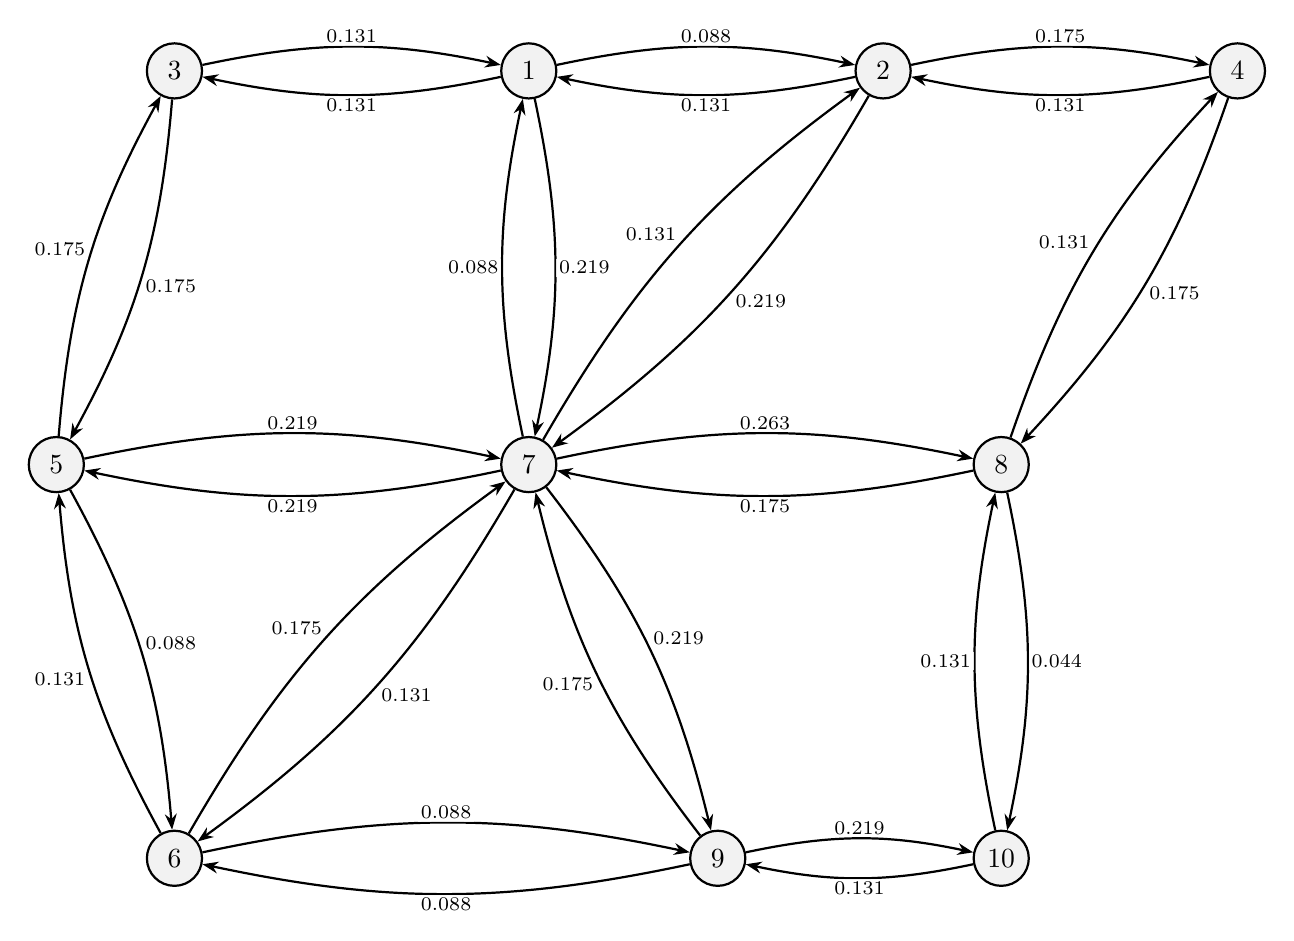
\begin{tikzpicture}[baseline, >={Stealth[length=2mm]},
  netnode/.style={circle, draw, thick, fill=gray!10, minimum size=7mm, inner sep=1pt},
  link/.style={thick},
  linklabel/.style={font=\scriptsize, inner sep=1pt, fill=white, fill opacity=0.85, text opacity=1}]
\node[netnode] (S1) at (6.000,10.000) {1};
\node[netnode] (S2) at (10.500,10.000) {2};
\node[netnode] (S3) at (1.500,10.000) {3};
\node[netnode] (S4) at (15.000,10.000) {4};
\node[netnode] (S5) at (0.000,5.000) {5};
\node[netnode] (S6) at (1.500,0.000) {6};
\node[netnode] (S7) at (6.000,5.000) {7};
\node[netnode] (S8) at (12.000,5.000) {8};
\node[netnode] (S9) at (8.400,0.000) {9};
\node[netnode] (S10) at (12.000,0.000) {10};
\draw[link, ->] (S1) to[bend left=12] node[linklabel, auto] {0.088} (S2);
\draw[link, ->] (S1) to[bend left=12] node[linklabel, auto] {0.131} (S3);
\draw[link, ->] (S1) to[bend left=12] node[linklabel, auto] {0.219} (S7);
\draw[link, ->] (S2) to[bend left=12] node[linklabel, auto] {0.131} (S1);
\draw[link, ->] (S2) to[bend left=12] node[linklabel, auto] {0.175} (S4);
\draw[link, ->] (S2) to[bend left=12] node[linklabel, auto] {0.219} (S7);
\draw[link, ->] (S3) to[bend left=12] node[linklabel, auto] {0.131} (S1);
\draw[link, ->] (S3) to[bend left=12] node[linklabel, auto] {0.175} (S5);
\draw[link, ->] (S4) to[bend left=12] node[linklabel, auto] {0.131} (S2);
\draw[link, ->] (S4) to[bend left=12] node[linklabel, auto] {0.175} (S8);
\draw[link, ->] (S5) to[bend left=12] node[linklabel, auto] {0.175} (S3);
\draw[link, ->] (S5) to[bend left=12] node[linklabel, auto] {0.088} (S6);
\draw[link, ->] (S5) to[bend left=12] node[linklabel, auto] {0.219} (S7);
\draw[link, ->] (S6) to[bend left=12] node[linklabel, auto] {0.131} (S5);
\draw[link, ->] (S6) to[bend left=12] node[linklabel, auto] {0.175} (S7);
\draw[link, ->] (S6) to[bend left=12] node[linklabel, auto] {0.088} (S9);
\draw[link, ->] (S7) to[bend left=12] node[linklabel, auto] {0.088} (S1);
\draw[link, ->] (S7) to[bend left=12] node[linklabel, auto] {0.131} (S2);
\draw[link, ->] (S7) to[bend left=12] node[linklabel, auto] {0.219} (S5);
\draw[link, ->] (S7) to[bend left=12] node[linklabel, auto] {0.131} (S6);
\draw[link, ->] (S7) to[bend left=12] node[linklabel, auto] {0.263} (S8);
\draw[link, ->] (S7) to[bend left=12] node[linklabel, auto] {0.219} (S9);
\draw[link, ->] (S8) to[bend left=12] node[linklabel, auto] {0.131} (S4);
\draw[link, ->] (S8) to[bend left=12] node[linklabel, auto] {0.175} (S7);
\draw[link, ->] (S8) to[bend left=12] node[linklabel, auto] {0.044} (S10);
\draw[link, ->] (S9) to[bend left=12] node[linklabel, auto] {0.088} (S6);
\draw[link, ->] (S9) to[bend left=12] node[linklabel, auto] {0.175} (S7);
\draw[link, ->] (S9) to[bend left=12] node[linklabel, auto] {0.219} (S10);
\draw[link, ->] (S10) to[bend left=12] node[linklabel, auto] {0.131} (S8);
\draw[link, ->] (S10) to[bend left=12] node[linklabel, auto] {0.131} (S9);
\end{tikzpicture}
\end{adjustbox}\end{center}

\begin{center}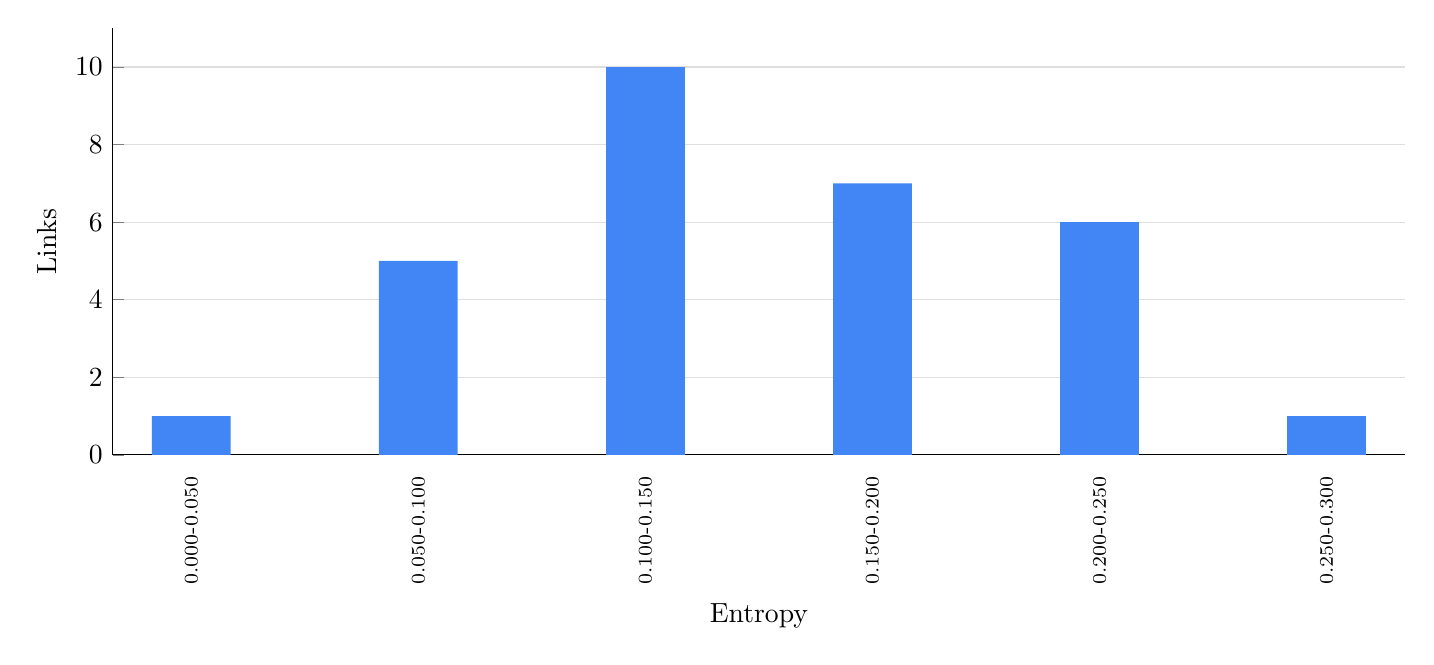
\begin{tikzpicture}
\begin{axis}[
  ybar, bar width=1.000cm, width=18.000cm, height=7cm,
  ymin=0, ymajorgrids, grid style={gray!25}, axis lines*=left,
  enlarge x limits={abs=1.000cm}, xtick=data, major x tick style={draw=none},
  x tick label style={rotate=90, font=\scriptsize, /pgf/number format/1000 sep=},
  legend style={at={(0.5,-0.3)}, anchor=north, legend columns=-1, draw=none},
  ylabel={Links},
  xlabel={Entropy},
  symbolic x coords={0.000-0.050,0.050-0.100,0.100-0.150,0.150-0.200,0.200-0.250,0.250-0.300,0.300-0.350,0.350-0.400,0.400-0.450,0.450-0.500,0.500-0.550,0.550-0.600,0.600-0.650,0.650-0.700,0.700-0.750,0.750-0.800,0.800-0.850,0.850-0.900,0.900-0.950,0.950-1.000}]
\addplot[fill={rgb,255:red,66;green,133;blue,244}, draw=none] coordinates {(0.000-0.050,1.000) (0.050-0.100,5.000) (0.100-0.150,10.000) (0.150-0.200,7.000) (0.200-0.250,6.000) (0.250-0.300,1.000) };
\end{axis}
\end{tikzpicture}\end{center}

\end{document}
